%%%%%%%%%%%%%%%%%%%%%
% 4章
%%%%%%%%%%%%%%%%%%%%%
\chapter{ヒューリスティクスを用いた手法} \label{chapter:4}

本章では,選挙区割問題を解くヒューリスティクスを作り,
その解から得られた選挙区の人口上限と下限を用いて,
ZDD構築を効率化する手法について提案する.

\section{概要}

\ref{chapter:3}章の人口制約付きZDD構築アルゴリズムでは,
パラメータとして部分グラフの重み上限$U$,下限$L$を用いた.
これを,許容格差定数$r$を使わず,ヒューリスティクスの解から,
最適解にできるだけ近い$U$,$L$を定義する.
$U$,$L$が最適解に近くなればなるほど,ZDDの構築時に,
最適解でない解候補の枝刈りの回数が多くなる.
その結果,従来手法に比べて
メモリの使用量の減少及び計算時間の短縮が期待できる.
提案手法の全体像を図\ref{heuristics}に記した.

\begin{figure}[htbp]
  \centering
  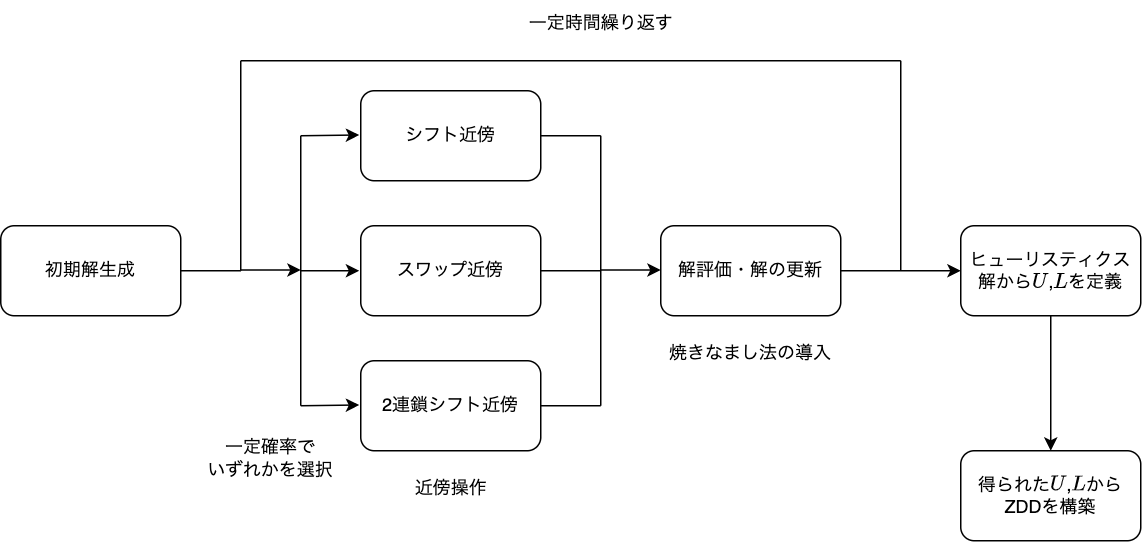
\includegraphics[scale=0.39]{img/heuristics.png}
  \caption{ヒューリスティクスを用いた提案手法}
  \label{heuristics}
\end{figure}



\section{初期解生成}

初期解は,幅優先探索を

\section{近傍操作}

\subsection{シフト近傍}

\begin{figure}[htbp]
  \centering
  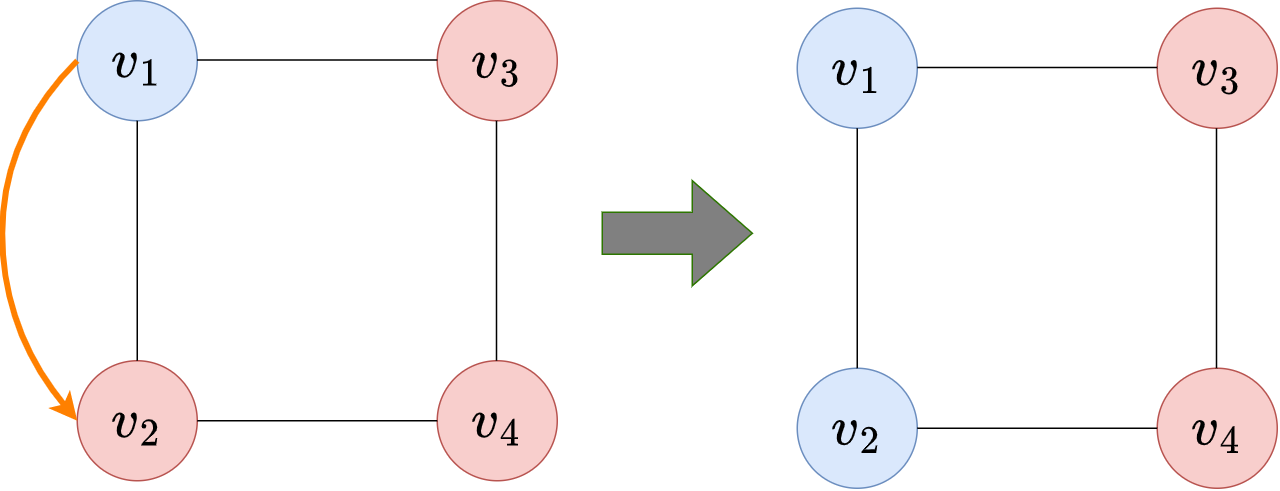
\includegraphics[scale=0.2]{img/shift-neighbor.png}
  \caption{シフト近傍}
  \label{shift-neighbor}
\end{figure}

\subsection{スワップ近傍}

\begin{figure}[htbp]
  \centering
  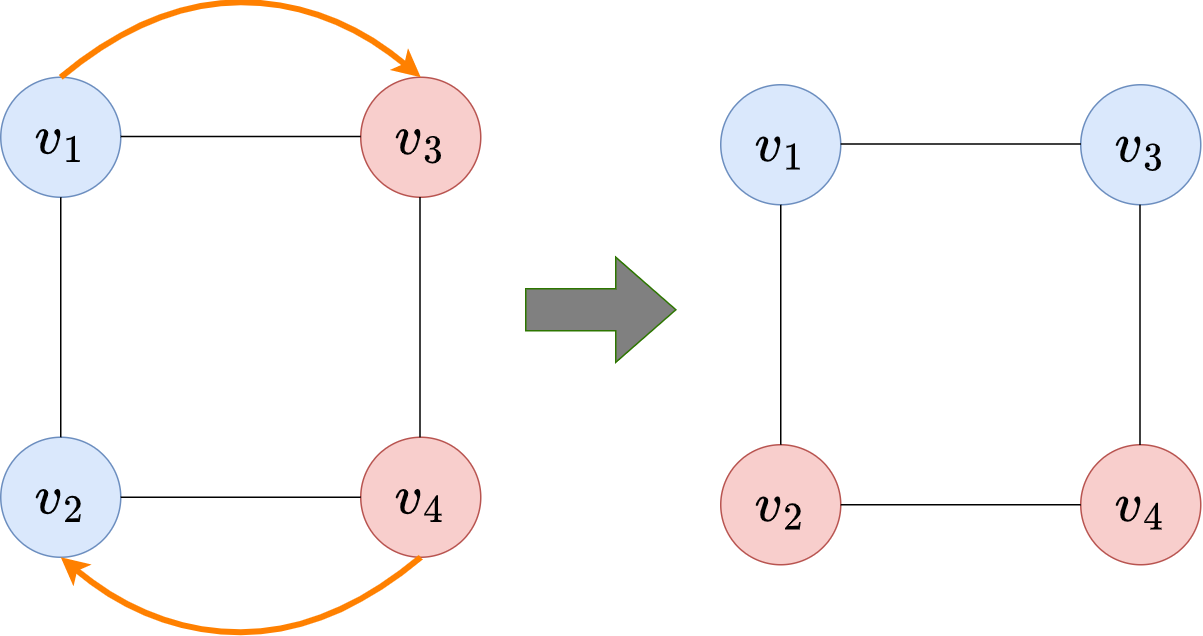
\includegraphics[scale=0.2]{img/swap-neighbor.png}
  \caption{スワップ近傍}
  \label{swap-neighbor}
\end{figure}

\subsection{2連鎖シフト近傍}

\begin{figure}[htbp]
  \centering
  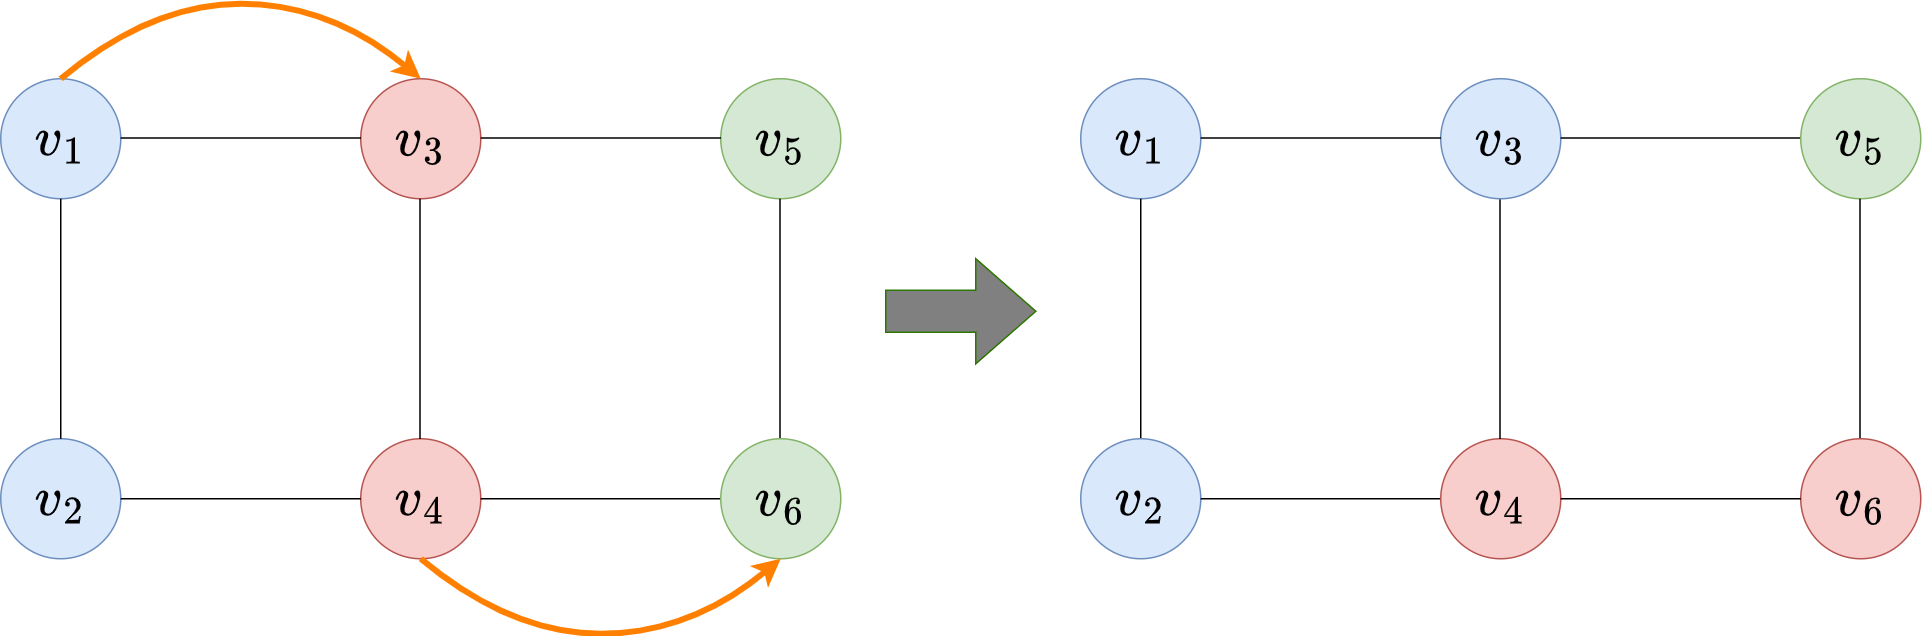
\includegraphics[scale=0.2]{img/chain-neighbor.png}
  \caption{2連鎖シフト近傍}
  \label{chain-neighbor}
\end{figure}

\section{焼きなまし法}

